\section{UI/UX Design}

The application has a streamlined user interface with a single window navigating between different views to ensure an intuitive and user-friendly experience. Below is the flow of UI/UX interactions:

\subsection{Initial Session Start}
The application starts with a view prompting the user to begin an ARKit session. This session initializes plane detection and world tracking. The interface provides visual indicators to guide the user during this setup phase. (Figure \ref{fig:ui_session_start} shows the UI at this stage.)
\begin{figure}[h!]
    \centering
    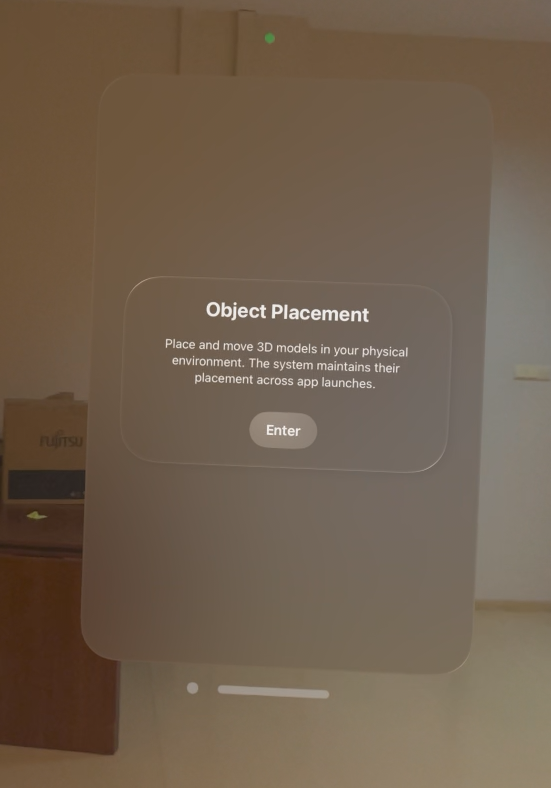
\includegraphics[width=0.4\textwidth]{session_start_ui.png} % Replace with your image file name
    \caption{UI for starting the ARKit session.}
    \label{fig:ui_session_start}
\end{figure}
\subsection{Object Selection Menu}
After initializing the session, the user is directed to an object selection menu. In this view:
\begin{itemize}
    \item The user selects an object from the available options.
    \item When an object is clicked, the \texttt{selectedObject} state is updated.
    \item The selected object is prepared for placement. (Figure \ref{fig:ui_object_selection} shows the object selection menu.)
\end{itemize}
\begin{figure}[h!]
    \centering
    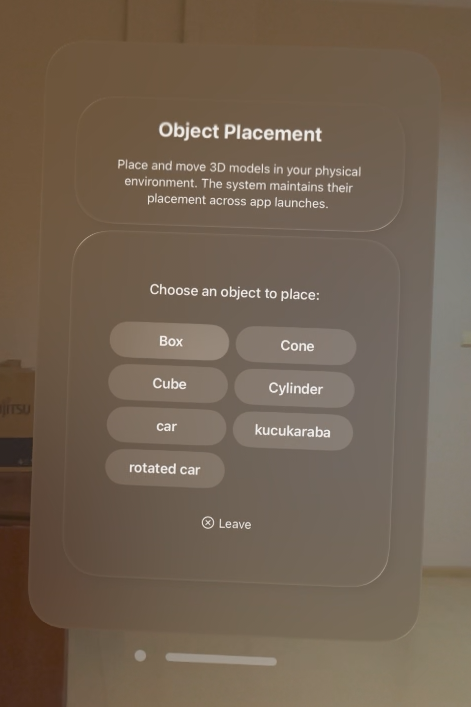
\includegraphics[width=0.4\textwidth]{object_selection_ui.png} % Replace with your image file
    \caption{Object selection menu UI.}
    \label{fig:ui_object_selection}
\end{figure}

\subsection{Initial Object Placement}
During the initial placement of the selected object:
\begin{itemize}
    \item Placement tooltips are displayed to guide the user on positioning the object accurately.
    \item Visual aids ensure the user understands how to interact with the AR environment. (Figure \ref{fig:ui_initial_placement} shows the placement tooltip.)
\end{itemize}
\begin{figure}[h!]
    \centering
    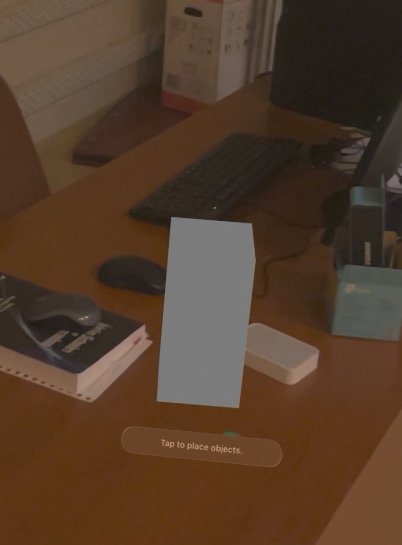
\includegraphics[width=0.4\textwidth]{object_placement_tooltips.png} % Replace with your image file
    \caption{Placement tooltips during initial object placement.}
    \label{fig:ui_initial_placement}
\end{figure}


\subsection{Object Interaction View}
If there is already a placed object, the application navigates directly to the object interaction view. In this view:
\begin{itemize}
    \item The user can perform repositioning, inspection, or removal of the placed object. The interface displays three buttons for these actions, as shown in Figure \ref{fig:ui_three_buttons}.
    \begin{figure}[h!]
        \centering
        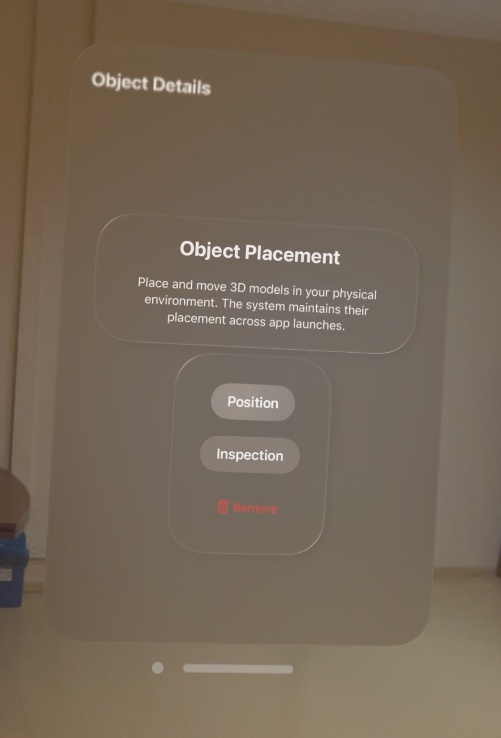
\includegraphics[width=0.39\textwidth]{three_buttons_ui.png} % Replace with the actual file name
        \caption{UI showing the three buttons for repositioning, inspection, and removal.}
        \label{fig:ui_three_buttons}
    \end{figure}
    \clearpage
    \item Three buttons allow the user to activate these actions:
    \begin{itemize}
        \item \textbf{Repositioning:} Includes rotation, left/right movement, and forward/backward movement. The user can use pinch and drag gestures (thumb and index finger) to perform the action. Only one action can be performed at a time. (Figure \ref{fig:ui_repositioning} shows the repositioning process.)
        \begin{figure}[h!]
            \centering
            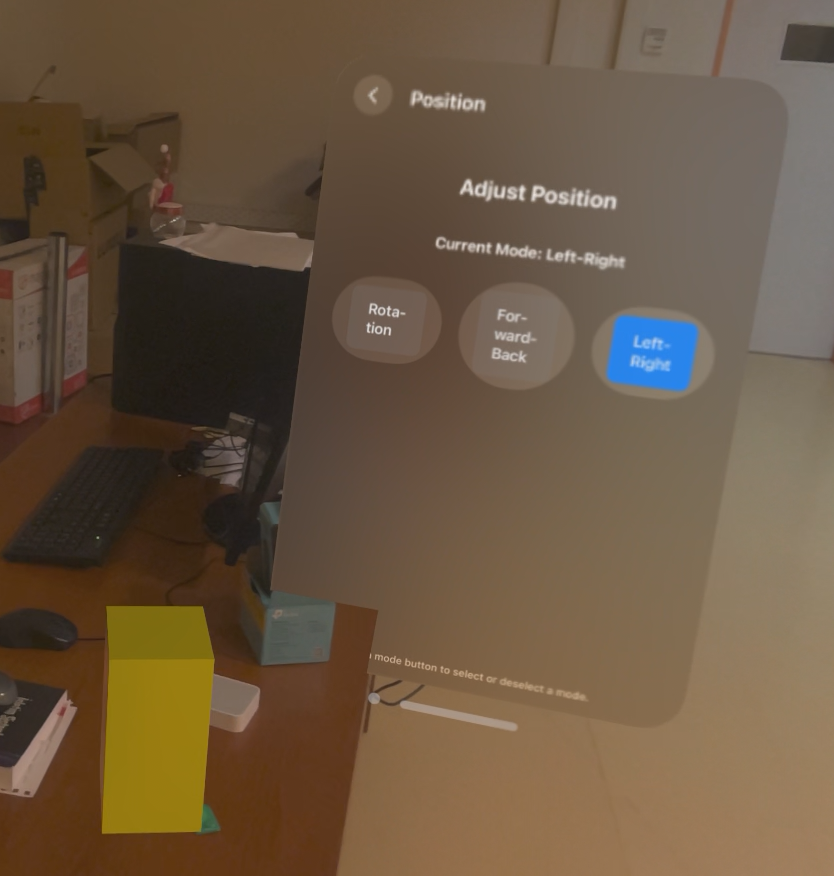
\includegraphics[width=0.6\textwidth]{repositioning_ui.png} % Replace with the actual file name
            \caption{Repositioning the object using pinch and drag gestures.}
            \label{fig:ui_repositioning}
        \end{figure}
        \item \textbf{Inspection:} Inspection points are UI buttons attached to the placed object. These points activate only in the inspection view. In addition, the inspection view includes a \textbf{Generate Report} button, allowing the user to extract detailed quality analysis reports based on the performed inspections. (Figure \ref{fig:ui_inspection_view} shows the inspection view.)
        \clearpage
        \begin{figure}[h!]
            \centering
            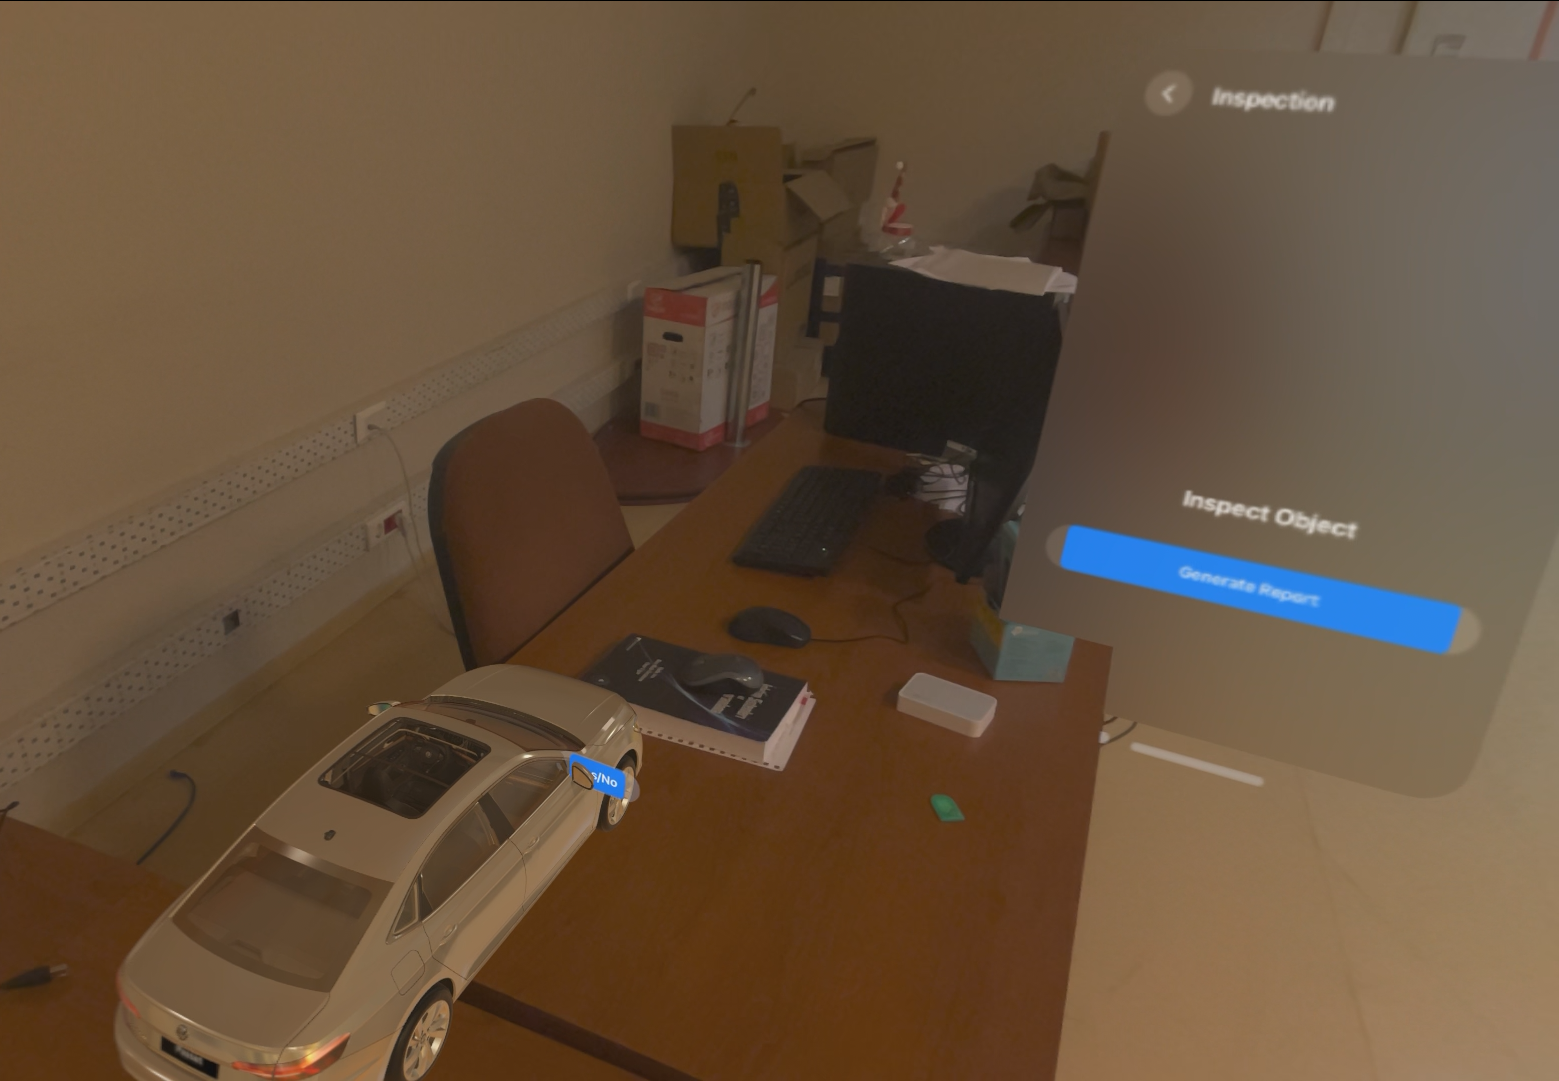
\includegraphics[width=0.8\textwidth]{inspection_view_ui.png} % Replace with the actual file name
            \caption{Inspection view showing active inspection points.}
            \label{fig:ui_inspection_view}
        \end{figure}
        \item \textbf{Removal:} To remove the placed object, the user presses the remove button. A confirmation popup appears to ensure the action is intentional. (Figure \ref{fig:ui_remove_popup} shows the removal confirmation popup.)
        \begin{figure}[h!]
            \centering
            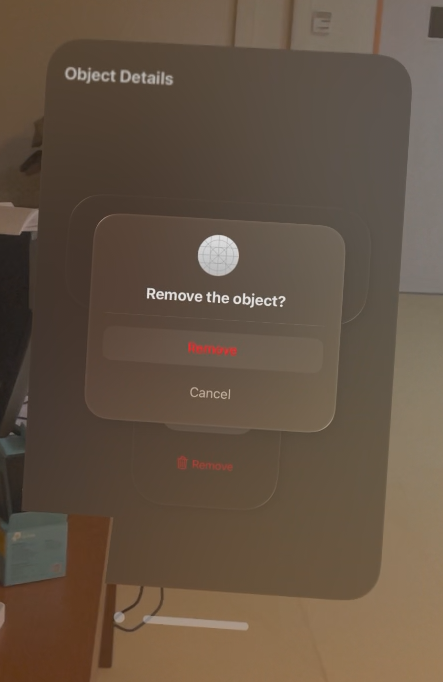
\includegraphics[width=0.4\textwidth]{remove_popup_ui.png} % Replace with the actual file name
            \caption{Confirmation popup for removing the placed object.}
            \label{fig:ui_remove_popup}
        \end{figure}
    \end{itemize}
\end{itemize}

\subsection{Inspection Detail View}
When an inspection point is clicked, the application navigates to the inspection detail view:
\begin{itemize}
    \item A question specific to the inspection point is displayed, which can be one of the following:
    \begin{itemize}
        \item Yes/No question.
        \item Count input.
        \item Description input.
    \end{itemize}
    \item The user provides the required input or feedback. (Figure \ref{fig:ui_inspection_detail} shows the inspection detail view.)
\end{itemize}

\begin{figure}[h!]
    \centering
    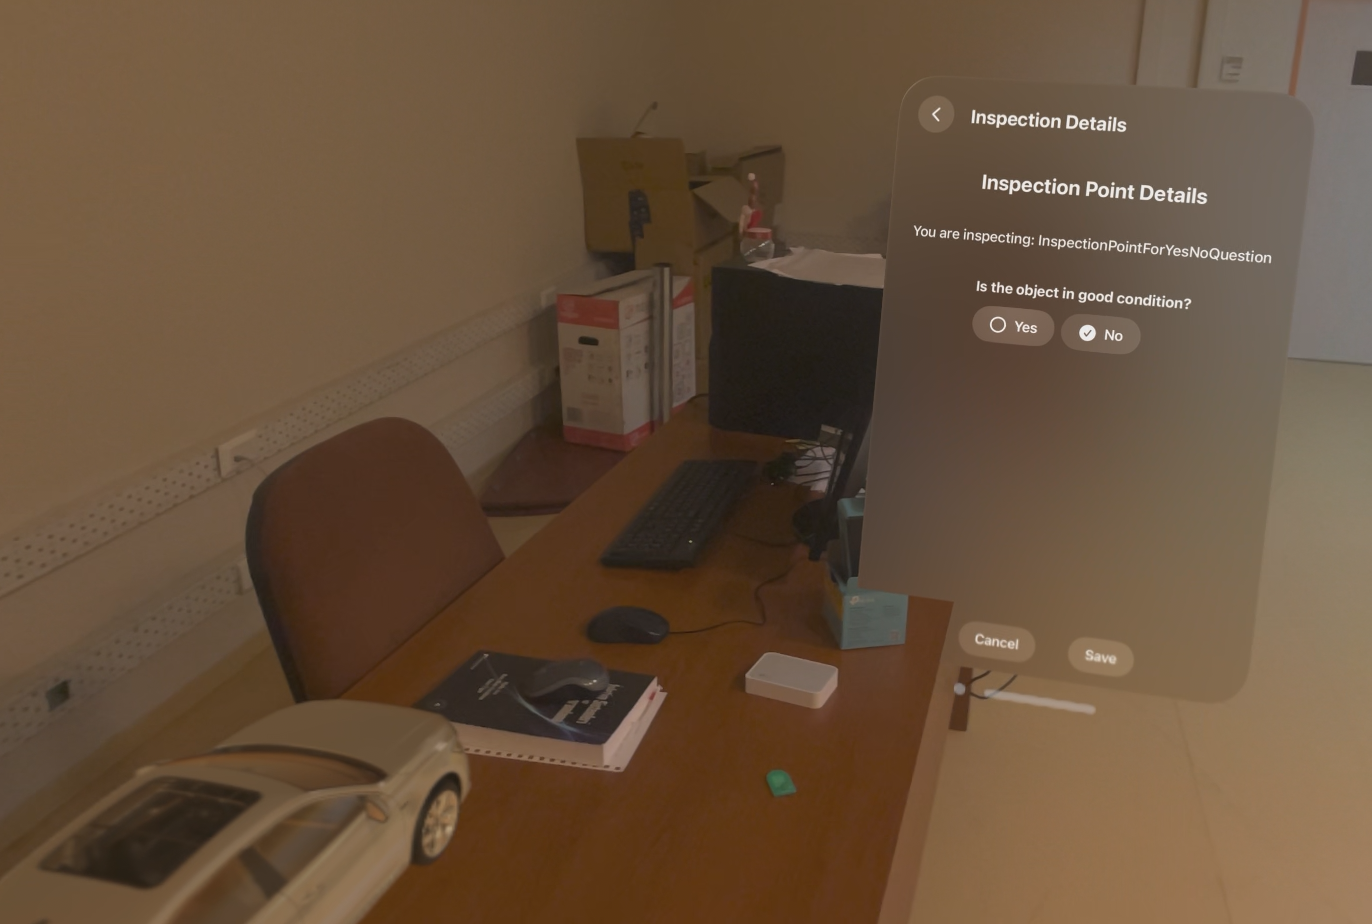
\includegraphics[width=0.8\textwidth]{inspection_detail_ui.png} % Replace with your actual file name
    \caption{Inspection detail view showing specific question types and input fields.}
    \label{fig:ui_inspection_detail}
\end{figure}
